% Chapter Template

\chapter{Procedura per l'estrazione di un modello da una TC e preparazione alla stampa 3D} % Main chapter title

\label{Chapter4} % Change X to a consecutive number; for referencing this chapter elsewhere, use \ref{ChapterX}
 
 %----------------------------------------------------


Avendo compreso i principi di diagnostica medica e di modellazione digitale, proseguiamo con un caso di utilizzo, che mostra come derivare un modello 3D da una serie di immagini diagnostiche. La procedura qui trattata serve a dare una panoramica sulle funzionalità principali dei software e sulle tecniche base di gestione delle immagini e dei modelli con l'obiettivo di fornire un flusso di lavoro generico e alcuni approfondimenti su eventuali variazioni di questo per la risoluzione ottimale di casi specifici.\\
Il caso qui presentato mostra come ottenere un modello di una mandibola e come prepararlo alla stampa. La procedura presentata si adatta bene all'estra\-zio\-ne di modelli di tessuti con forte contrasto rispetto a quelli circostanti, come il tessuto osseo nelle TC.

\section{Anonimizzazione delle immagini}
Prima di iniziare al lavorare con le immagini dobbiamo fare in modo che queste non contengano dati sensibili con i quali si possa risalire all'identità del paziente. In questo caso useremo il software open-source \emph{DICOM Confidential}, sviluppato dal team \emph{Data Intensive Research dell'Università di Edimburgo} \parencite{Reference46} \parencite{Reference146}. Il software permette di caricare una cartella contenente le immagini, che vengono quindi processate secondo le direttive inserite.\\
All'apertura del software ci si presenta l'interfaccia grafica (GUI).
Qui è possibile caricare la cartella contenente il set da anonimizzare.\\
È possibile impostare le voci \emph{Policy URI} e \emph{Workflow file}. Queste sono le indicazione sul workflow da eseguire e sulle operazioni di anonimizzazione da compiere sulle immagini. Il software all'installazione fornisce dei template standard da utilizzare. Questi possono essere modificati secondo le esigenze del caso, e si trovano nel percorso \path |C: Userpath\DICOM Confidential| (dove \path |C: Userpath\DICOM Confidential\| è la cartella in cui il software è stato installato).\\
La path di output è \path |C: Userpath\DICOM Confidential\data\ANONYMISED|. Usando i file standard di configurazione,  ogni set anonimizzato verrà riconosciuto dal software per l'apertura delle DICOM come appartenente all'unico paziente "ANONYMISED", a cui verranno aggiunti tutti gli studi anonimizzati. Da tenere in considerazione durante l'organizzazione del sistema.
\begin{figure} [h]
	\centering
	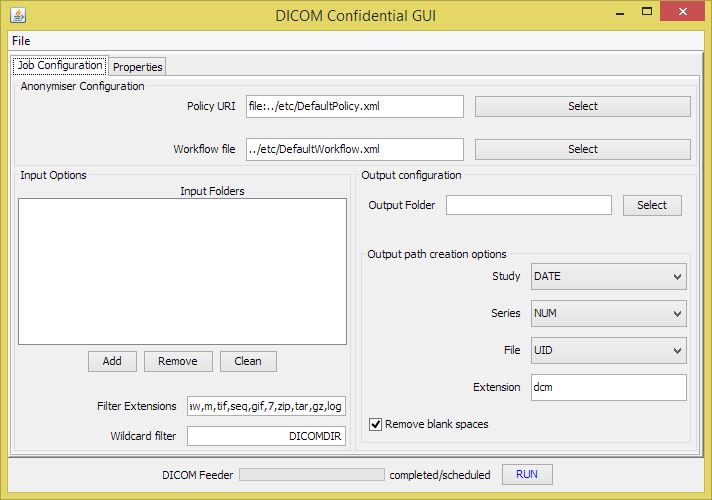
\includegraphics[width=0.9\textwidth, keepaspectratio]{gui_dicomConf}
    \caption{Schermata principale del software \emph{DICOM Confidential}}
    \label{fig:gui_dicomConf}
\end{figure}

\section{Immagini già anonimizzate}
È possibile scaricare dataset già anonimizzati dal \emph{Cancer Imaging Archive} \parencite{Reference47}, un database curato dal \emph{The National Cancer Institute} (NCI) e dalla \emph{University of Arkansas for Medical Sciences} (UAMS) per favorire la ricerca multisciplinare \parencite{Reference48}, assieme ai dataset del \emph{Cancer Genome Atlas} \parencite{Reference49}.\\
Sono li disponibili svariati studi effettuati con le diverse tecniche di imaging disponibile, che danno la possibilità di approfondire l'analisi di vari segmenti corporei e delle patologie oncologiche che vi si possono presentare.\\
Per utilizzare le immagini vanno seguite le semplici procedure descritte sul sito. Una volta ottenuti i dati, questi possono essere caricati direttamente sul software di visualizzazione.
                             
\section{Apertura delle immagini}
Le immagini ottenute possono essere quindi caricate su 3d Slicer per la visualizzazione e l'elaborazione. Useremo un set di immagini scaricato dal portale \emph{Cancer Imaging Archive}, situato all'interno della collezione \path |TCGA - HNSC , Subject ID: TGCA-BA-6868|, scansione \emph{Neck BW Axial}.\\
Il software si avvale del modulo \emph{DICOM} \parencite{Reference50} per caricare e gestire i set di immagini diagnostiche. Il modulo \emph{Volume rendering} può essere utilizzato per visualizzare un rendering delle immagini.\\
Con il modulo \emph{Crop Volume} è possibile tagliare la parte di volume di nostro interesse (Region of Interest, ROI), per alleggerire il computer da dati che al momento non sono necessari, il che tornerà molto utile più avanti quando lavoreremo con i modelli. In questo esempio vogliamo creare un modello di \emph{\textbf{osso mandibolare}}, orientiamo quindi la ROI in modo che contenga le ossa mascellari e applichiamo la modifica.
\begin{figure}[h]
\centering
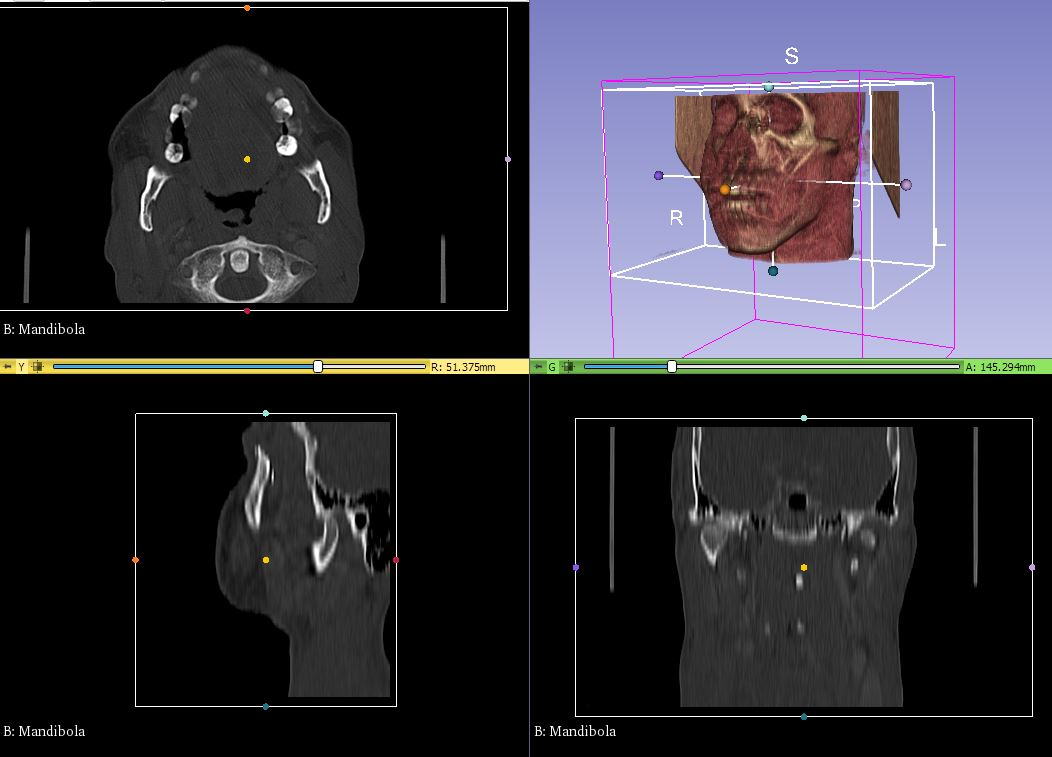
\includegraphics[width=0.8\textwidth, keepaspectratio]{crop1}
\caption{crop effettuato sulle immagini per selezionare le arcate mascellari}
\label{fig:crop}
\end{figure}

\section{Segmentazione e creazione modello}
Possiamo quindi iniziare la segmentazione, utilizzando il modulo \emph{Segment Editor}. Questo modulo contiene diversi strumenti che ci permettono di evidenziare le aree delle immagini che ci interessano. Dato che vogliamo estrarre il modello di un osso, la mandibola, un metodo veloce è quello di utilizzare il \emph{range di densità del tessuto osseo} per evidenziare rapidamente la regione di nostro interesse. Quindi col il pulsante \emph{Add} aggiungiamo un segmento e selezioniamo lo strumento \emph{Threshold} che ci permette appunto di selezionare un range di densità da evidenziare. Lo strumento \emph{Data Probe} in basso a sinistra ci da informazioni sul punto dell'immagine in cui si trova la punta del mouse, e contiene una voce che indica la densità nel punto.\\
Nella scelta del threshold cerchiamo un compromesso tra completezza nella cattura dei particolari e pulizia dell'immagine. Abbiamo la possibilità di effettuare una rifinitura manuale della segmentazione, quindi possiamo permetterci di lasciare qualche area non selezionata dal threshold per avere una maggiore pulizia tra le parti da segmentare. Consideriamo che le aree selezionate, per essere trattate come aree singole devono essere separate, tranne nel caso in cui si usa un segmento per ciascuna area; in quel caso i voxel della selezione possono essere adiacenti senza unire i volumi in un unico oggetto.
Importante è comunque selezionare al meglio le aree di interesse, e nella TC che stiamo segmentando un punto delicato per la corretta separazione della mandibola si trova nell'area dei condili, dove la selezione risulta continua con quella della parete anteriore della cavità glenoidea dell'osso temporale. Un altro punto che potrebbe andar separato è la regione posteriore dell'arcata dentaria, al livello del piano occlusale, dove i denti della mandibola potrebbero essere uniti agli antagonisti.
\begin{figure}[h]
\centering
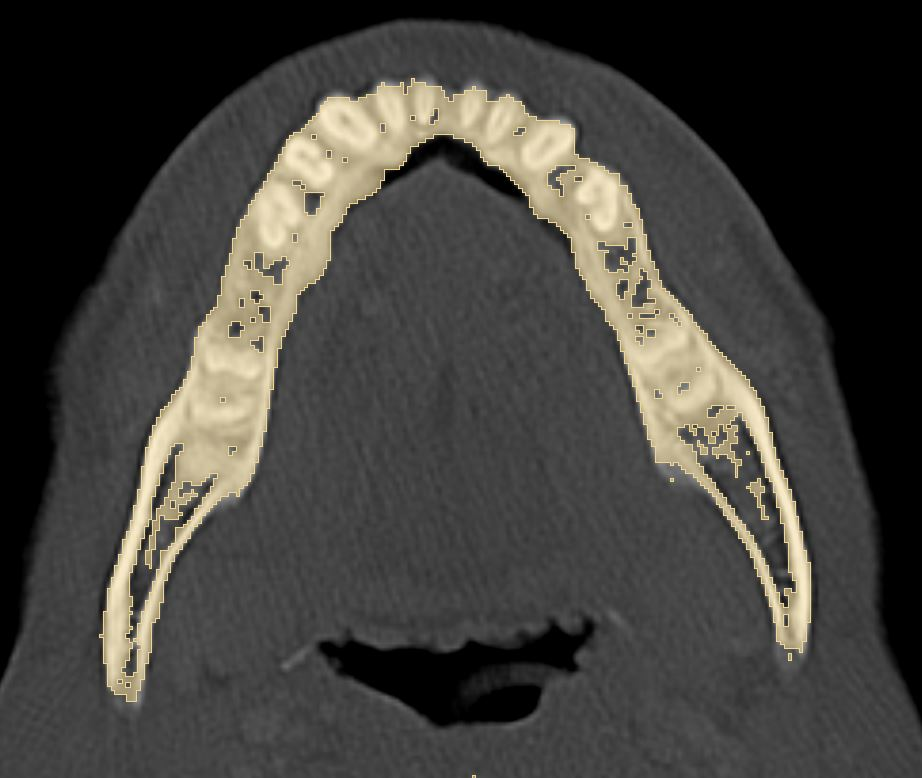
\includegraphics[width=0.7\textwidth, keepaspectratio]{origin_label}
\caption{Selezione di osso mandibolare ed elementi dentari inferiori; \emph{threshold} 220 - 3071 HU; rimozione di gruppi di voxel di piccole dimensioni: \emph{Island}>\emph{remove small island (minimum voxel = 1000)}.}
\label{fig:origin_label}
\end{figure}
\\
Applicato il threshold vediamo che sui voxel che rientrano nel range di densità selezionato è stata creata una maschera. Questa maschera va modificata manualmente, aggiungendo eventuali aree mancanti e separando le parti di nostro interesse da quelle adiacenti. Cliccando sul bottone \emph{Show 3D} possiamo vedere l'anteprima del modello creato dalla segmentazione; questa opzione è utile per vedere se le aree selezionate corrispondono al modello che vogliamo ottenere, ma durante la modifica della maschera è meglio disattivare l'opzione per risparmiare risorse, ed attivarla solo quando necessario.\\
La rimozione delle aree di contatto tra due parti, nel nostro caso il condilo mandibolare e il condilo del temporale, vene eseguita in 3D Slicer per velocizzare la processazione successiva del modello. Si sarebbe potuto creare un modello già dopo l'uso del threshold, ma la separazione di due modelli in software come Blender è più lunga e macchinosa della semplice selezione/deselezione dei voxel che si può eseguire in 3D Slicer.\\
\begin{figure}[h]
\centering
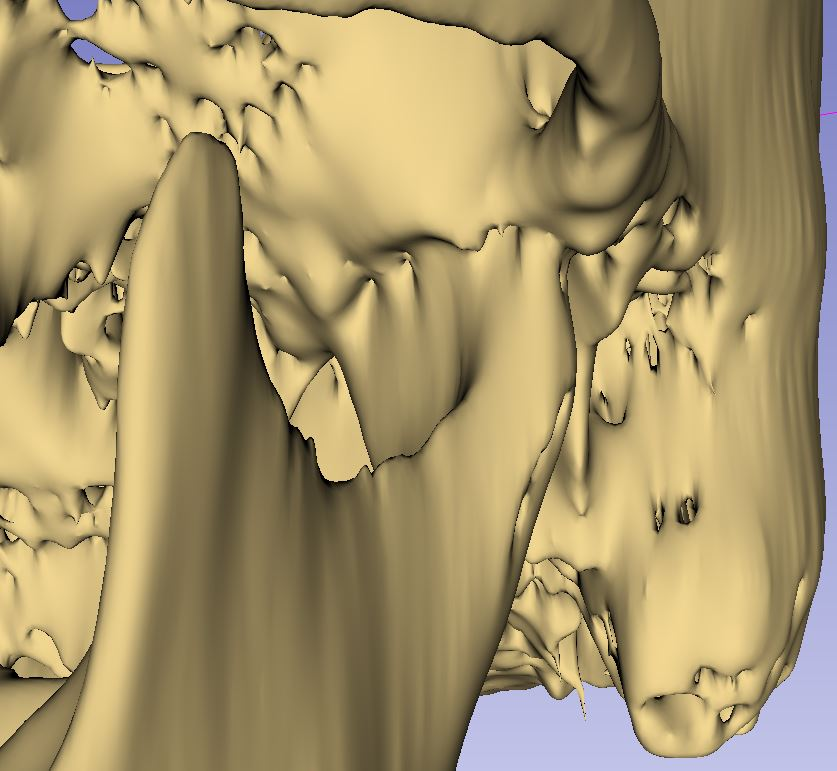
\includegraphics[width=0.7\textwidth, keepaspectratio]{fuso_condi}
\caption{Ricostruzione 3D della segmentazione eseguita con threshold. Si nota che la mandibola risulta fusa all'osso temporale.}
\label{fig:fuso_condi}
\end{figure}
Puntiamo quindi ad ottenere da Slicer un modello 3D il più preciso e pulito possibile, per ridurre la durata degli step successivi, ma anche per creare dataset di segmentazioni di qualità, che sono utili per altri scopi (data analysis, training set per Neural Network).\\
Lo strumento \emph{Erase} permette di rimuovere dalla maschera i voxel che non ci serve selezionare.\\
Lo strumento \emph{Paint} permette di colorare voxel di interesse che non sono strati selezionati dal threshold.\\
Dopo aver eseguito la rifinitura possiamo utilizzare lo strumento \emph{Island} con l'opzione \emph{Keep Selected Island} attivata; cliccando sulla maschera di selezione della mandibola. Se questa è sepatata dal resto del cranio avremo effettuato correttamente la separazione, che possiamo controllare visualizzando il modello col bottone \emph{Show 3D}. Se desideriamo anche il modello del resto del cranio, possiamo cliccare sul bottone \emph{Undo} per tornare indietro di uno step e recuperare l'isola contenente la mascella e parte del cranio.\\
Possiamo creare un segmento dalla porzione di maschera del cranio. Aggiungiamo un segmento dal bottone \emph{Add} e lo selezioniamo; usando lo strumento \emph{Island} con l'opzione \emph{Add Selected Island} clicchiamo sulla maschera del cranio e questa sarà aggiunta al nuovo segmento. Separare gli oggetti in segmenti fa perdere la relazione spaziale tra le parti, quindi se è necessario che le parti siano in una particolare posizione tra loro devono essere selezionata l'opzione \emph{Merge into single file} per esportare in un unico file. È poi possibile separare questo unico modello nelle sue due componenti col software Blender. \\
Passiamo quindi al modulo \emph{Segmentation}, dove dal menù a sinistra troviamo in basso la finestra \emph{Export to File}; selezioniamo la cartella di destinazione ed esportiamo i file in formato .stl.
\begin{figure}[h]
\centering
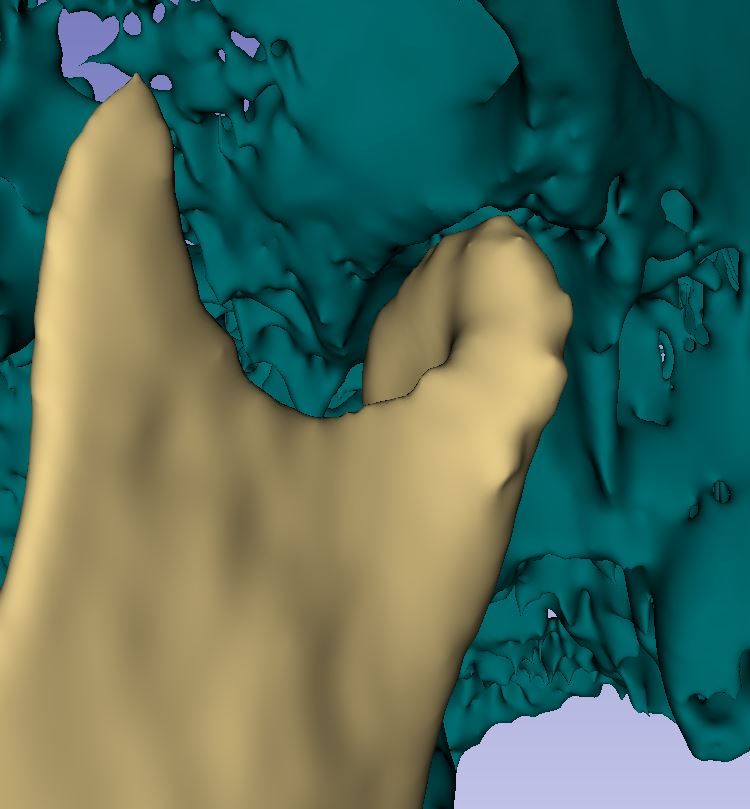
\includegraphics[width=0.7\textwidth, keepaspectratio]{sepa_condi}
\caption{Mandibola separata dall'osso temporale. La separazione è stata eseguita manualmente con gli strumenti erase e paint. Dopo la separazione sono stati creati un Segmento per la mandibola (giallo) ed uno per il cranio (blu).}
\label{fig:sepa_condi}
\end{figure}

\section{Processazione del modello}
Importiamo il modello ottenuto in MeshMixer e all'interno del menù \emph{Analysis} selezioniamo lo strumento \emph{Inspector}. Questa funzione ha essenzialmente il compito di rilevare difetti che è necessario risolvere per avere un modello chiuso (\emph{manifold}) e di rimuovere componenti separate dalla mesh principale. È utile per preparare un modello per la stampa 3D, dove è necessario che il modello sia appunto chiuso, a tenuta stagna (\emph{watertight}). Questo tool è utile per la risoluzione di piccoli problemi alle mesh, ma situazioni più complesse potrebbero richiedere la riparazione manuale, effettuabile sia in questo software che con Blender e MeshLab.
\vspace{3cm}
\begin{figure}[h]
\centering
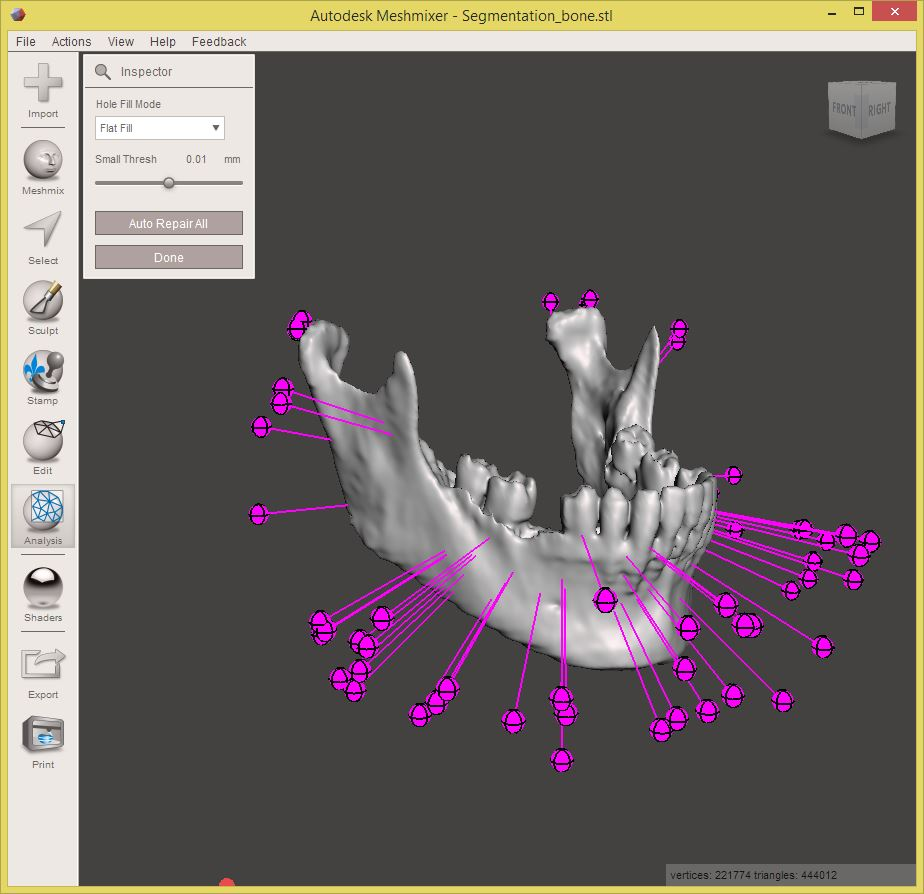
\includegraphics[width=0.8\textwidth, keepaspectratio]{inspector}
\caption{Strumento \emph{Inspector} in MeshMixer. Ogni indicatore viola può essere cliccato per riparare un difetto della mesh.}
\label{fig:inspector}
\end{figure}


Il modello può quindi essere esportato in Blender per effettuare uno smoothing. Nel menù \emph{Modificatori}  selezioniamo il modificatore \emph{Smooth}. Questa è una funzione che leviga la superficie dell'oggetto, provocandone una lieve diminuzione del volume. Nel menù dello strumento possiamo impostare il numero di passaggi del filtro sul modello; troviamo un compromesso tra levigatura e mantenimento delle dimensioni. Un altro modo per levigare la superficie è farlo manualmente, con gli strumenti di scultura \emph{sculpting} presenti sia in Blender che in MeshMixer.\\
Dopo aver levigato il modello lo ispezioniamo per valutarne la qualità; è possibile usare il software MeshLab per comparare due mesh. Nel nostro caso misureremo la differenza tra il modello originale e il modello ottenuto dopo 50 iterazioni del Modificatore \emph{smooth} in Blender. A modelli allineati l'uno con l'altro, la procedura consiste nell'usare il filtro Hausdorff Distance per valutare la distanza tra le due mesh \parencite{Reference90}, \parencite{Reference91}. Il software restituirà le misurazioni relative al campionamento della mesh.\\
\vspace{3cm}
\begin{figure}[h]
\centering
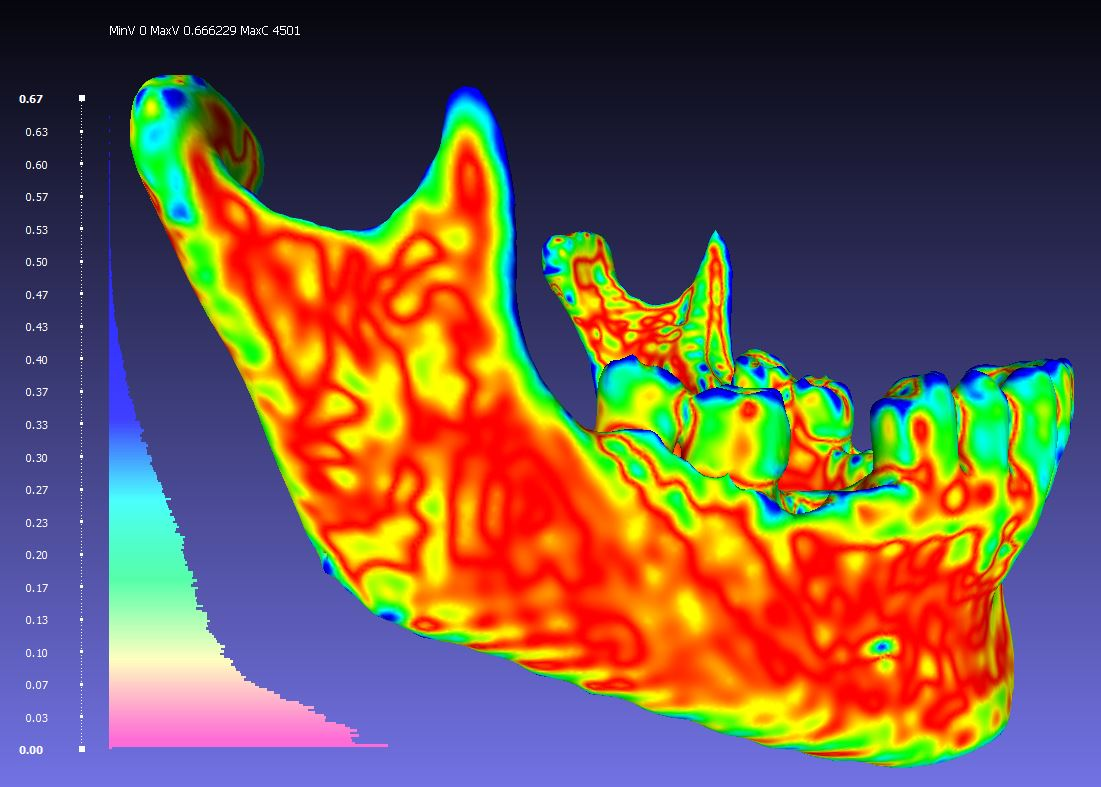
\includegraphics[width=0.8\textwidth, keepaspectratio]{hausdorff_smooth_clean}
\caption[LoF entry]{Valutazione della distanza di Hausdorff tra la mesh originale e la stessa mesh dopo 50 step di "Smooth" in Blender. La scala va da rosso (errore 0) a blu (errore massimo)}
\begin{lstlisting}
Hausdorff Distance computed
Sampled 4657134 pts (rng: 0) on smooth_clean_Segmentation_bone.stl
searched closest on clean_Segmentation_bone.stl
min: 0.000000; max: 0.695190; mean: 0.116956; RMS: 0.154653

Values w.r.t. BBox Diag (181.472809)
min: 0.000000; max: 0.003831; mean: 0.000644; RMS: 0.000852 
Applied filter Hausdorff Distance in 29689 msec

Quality Range: 0.000000 0.666229; Used (0.006929 0.335713)
percentile (5.000000 95.000000) 
Applied filter Colorize by vertex Quality in 51 msec
\end{lstlisting}

\label{fig:hausdorff_smooth_clean}
\end{figure}
\\
È poi possibile colorare la mesh per valutare visivamente la discrepanza con la mesh originale. Per fare questo dal menù \emph{Filter} selezioniamo \emph{Color Creation and Processing} --> \emph{Colorize by Vertex Quality}. Possiamo renderizzare l'istogramma dal menù \emph{Render} --> \emph{Show Quality Histogram}.\\
Teniamo presente che la scala colori va dal rosso al blu, dove il \emph{rosso} indica massima corrispondenza con la mesh originale, mentre il \emph{blu} indica una maggiore distanza dalla mesh originale. Il valore è indicato in unità del modello, in questo caso millimetri.\\
In alternativa a MeshMixer è possibile usare MeshLab per svolgere operazioni più avanzate sulle mesh.
Per rimuovere le regioni separate dalla mesh principale si fa uso dello strumento \emph{Filter} --> \emph{Cleaning and Reapiring} --> \emph{Remove Isolated Pieces (wrt. Faces Numbers)}, impostando il numero minimo di facce ad un livello abbastanza alto, in base al numero di facce mostrato nella tool-bar in basso.\\
Per ottenere una \emph{mesh 2-manifold} \parencite{Reference92}, \parencite{Reference93}, in termini pratici una \emph{mesh chiusa}: dal menù \emph{Filter} --> \emph{Cleaning and Repairing} utilizzare le funzioni: \emph{Remove Duplicate Faces}, \emph{Remove Duplicate Vertex}, \emph{Remove Unreferenced Vertices}, \emph{Remove Faces From Non Manifold Mesh}, \emph{Remove t-vertices From Non Manifold Edges}.\\ Questi comandi effettuano una pulizia della mesh, mentre per ricostruire la mesh 2-manifold usiamo il comando \emph{Filter} --> \emph{Remeshing, Semplification and Recostruction} --> \emph{Screened Poisson Surface Sampling} \parencite{Reference95}, \parencite{Reference96}.\\ Questa ricostruzione, pulita e 2-manifold, può essere usata per ulteriori elaborazioni. Eseguendo una valutazione della congruità della ricostruzione, si nota come la discrepanza con l'originale sia molto bassa.\\
\begin{figure}[h]
\centering
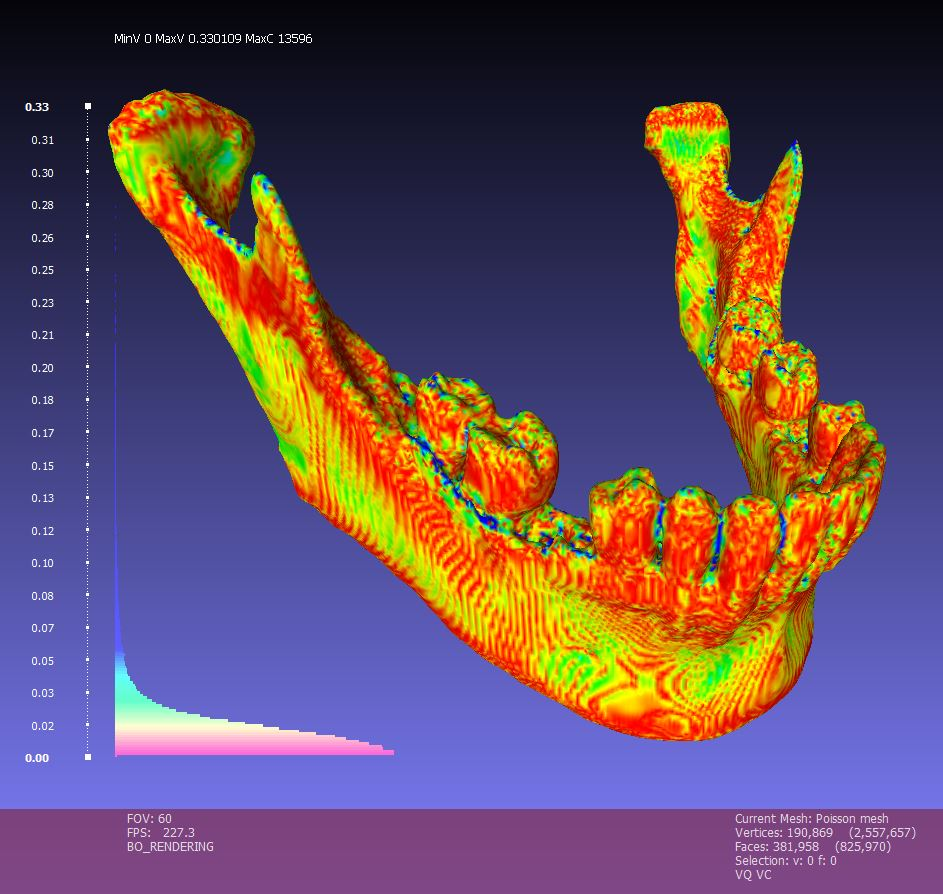
\includegraphics[width=0.8\textwidth, keepaspectratio]{noSeparate_poisson_clean_hausdorff}
\caption[LoF entry]{Calcolo della distanza di Hausdorff dopo l'applicazione dell'algoritmo \emph{Screened Poisson Surface Sampling}}
\begin{lstlisting}

Hausdorff Distance computed
Sampled 4195438 pts (rng: 0) on Poisson mesh searched 
closest on Segmentation_bone.stl
min : 0.000000 max 0.432402 mean : 0.019149 RMS : 0.031849

Values w.r.t. BBox Diag (182.226028)
min : 0.000000 max 0.002373 mean : 0.000105 RMS : 0.000175 
Applied filter Hausdorff Distance in 20254 msec
\end{lstlisting}

\label{fig:noSeparate_poisson_clean_hausdorff}
\end{figure}
\\

Possiamo effettuare un ulteriore controllo con lo strumento \emph{Inspector} di MeshMixer per valutare la necessità di ulteriori perfezionamenti alla mesh.
Il modello va quindi esportato in formato .stl per prepararlo alla stampa 3D.


\section{Slicing}
Il modello digitale della Mandibola è stato ricavato dalla TC e rifinito per assicurare un modello idoneo alla stampa. Effettueremo lo slicing del modello per mezzo del software Cura.
Carichiamo il modello è selezioniamo il \emph{Print Setup} voce \emph{Custom}, per avere la possibilità di regolare con precisione i parametri di stampa, che sono inizialmente nascosti e vanno attivati.\\
Le impostazioni da regolare dipendono da diverse variabili, tra cui:

\begin{itemize}
\item le caratteristiche della stampante;
\item le caratteristiche del modello da stampare;
\item il materiale di stampa;
\item l'accuratezza e le proprietà meccaniche attese dall'oggetto che ci si approccia a stampare.
\end{itemize}
	
Sono da tenere in considerazione anche le condizioni ambientali in cui si opera, perché ad esempio alcuni parametri possono cambiare tra una stampa eseguita in una stampante chiusa o in una aperta.\\
Fondamentale per un buon risultato di stampa è la calibrazione della stampante e la conoscenza delle specifiche di quest'ultima. Cura genererà le istruzioni di stampa per la stampante basandosi sulle specifiche della stampante che abbiamo inserito nel menu \emph{Printers} > \emph{Machine Settings}. Questi settaggi vengono spesso aggiornati con l'aggiunta dei dati delle stampanti più diffuse, ma per le stampanti autoassemblate i parametri vanno inseriti manualmente.\\
Con la stampante calibrata e le informazioni correttamente inserite in Cura, il modello verrà visualizzato nel software e verrà effettuato lo slicing con i parametri inseriti. Completata la procedura di slicing potremo vedere il modello strato per strato (\emph{Layer View}).
Il \emph{\textbf{G-code}} così ottenuto può essere utilizzato dalla stampante per produrre il modello.
\begin{figure}[t]
\centering
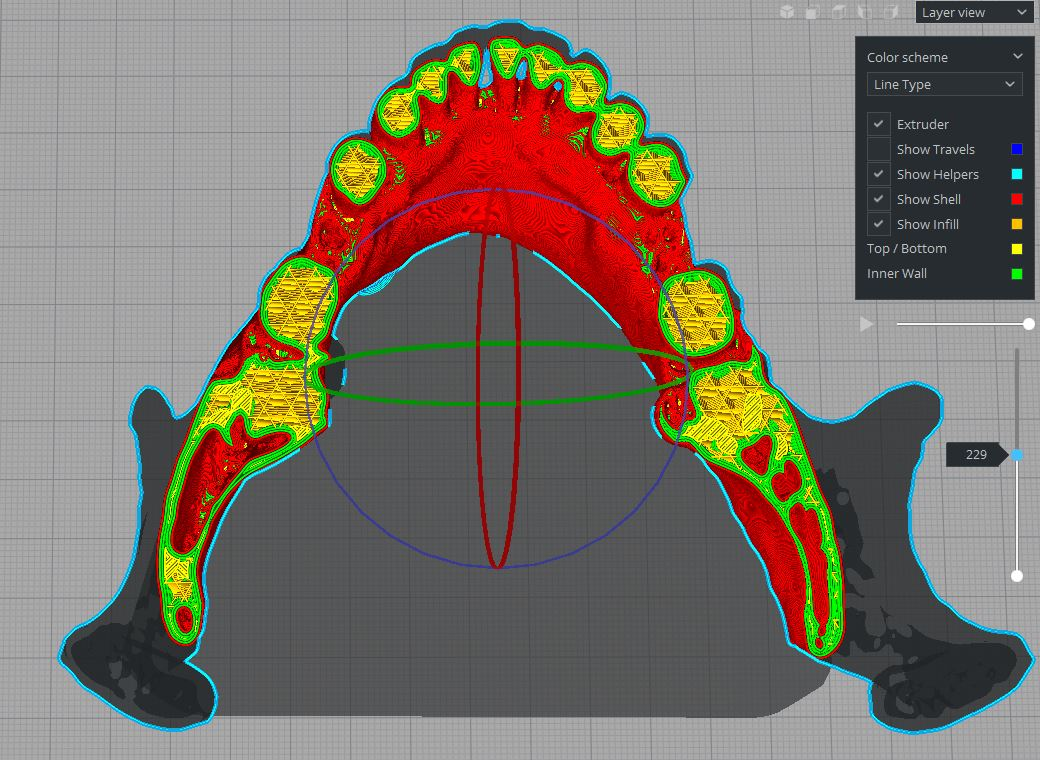
\includegraphics[width=\textwidth, keepaspectratio]{slicing}
\caption{Slicing della mandibola in Cura.}
\label{fig:slicing}
\end{figure}

